\section{Results}

\subsection{2025 thrombectomy performance statistics (from SSNAP)}

In 2025, 4.8\% of all emergency stroke admissions received MT. The use for ischaemic stroke was 5.6\%. The use for ischaemic stroke with a stroke severity (NIHSS) of 11+ was 22.1\%.

For ischaemic strokes with NIHSS 11+, the MT rate depending on the type of first admitting unit was:

\begin{itemize}
    \item First admitted to MT unit (do not require transfer for MT) = 24.7\%
    \item First admitted to IVT-only unit (require transfer for MT) = 16.5\%
    \item \textit{Summary}: MT rate for patients requiring transfer is 67\% of those not requiring transfer
\end{itemize}

The above analysis has informed our modelling: for scenarios including onward transfers for MT from IVT-only units, we have also modelled the effect of a 33\% MT loss for those transferred from an IVT-only unit.

The first arrival to thrombectomy times (median and quartiles) were:

\begin{itemize}
    \item First admitted to MT unit = 128 mins (95-183 mins)
    \item First admitted to IVT-only unit = 241 mins (182-308 mins)
    \item \textit{Summary}: 113 mins delayed MT (on average) when transfer required (includes transfer-related net delay and transport time)
\end{itemize}

\subsection{Clinical benefit of reperfusion treatment (modelled results)}

\subsubsection{Clinical benefit of current system}

In the current system (including new MT units in East Kent and Norwich), without reperfusion treatment the model predicts 26.5\% of LVO patients would achieve a good outcome (mRS 0-2 at 3-6 months). With IVT alone, this would increase to 32.4\% for treated LVO patients, and with IVT and MT there would be a further increase to 37.8\%. If all LVO patients attended their closest MT unit first (a \textit{mothership} model of care) 42.0\% of treated LVO patients would achieve a good outcome (mRS 0-2 at 3-6 months). Directing as many treatable LVO patients to their closest MT unit would maximise outcomes.

There is significant variation in clinical benefit by geography, even without loss of MT procedures for patients who first attend an IVT-only unit. Total travel time to an MT unit, including transfer time when required, ranges from 0 to 192 minutes (including a net non-travel time delay to MT of 60 minutes for transfer). The proportion of treated patients who achieve a good outcome (mRS 0-2 at 3-6 months) ranges from 31.8\% to 39.8\% in England (a benefit of treatment of between 5.4 and 13.3 percentage points increase in a good outcome, mRS 0-2 at 3-6 months). Those living closest to an MT unit have the greatest benefit from treatment, with the least benefit for those with the longest time to MT (a combination of travel time to their closest IVT-only unit, non-travel transfer-related delays, and the travel time from that IVT unit to the closest MT unit).

\subsubsection{Clinical benefit of planned system (2 additional MT units)}

We have compared the expected benefit of the current system (including new MT units in East Kent and Norwich) to the same system with the addition of MT units at Taunton and Worcester.

The addition of a new MT unit in Taunton potentially benefits a catchment population of 2,736 stroke admissions per year. The net improvement is expected to be about 2.9 additional good outcomes (mRS 0-2 at 3-6 months) if there is no loss of MT for patients first admitted to an IVT-only unit.

The addition of a new MT unit in Worcester potentially benefits a catchment population of 2,010 stroke admissions per year. The net improvement is expected to be about 2.7 additional good outcomes (mRS 0-2 at 3-6 months) if there is no loss of MT for patients first admitted to an IVT-only unit.

Improvement in outcomes is not even across the population who may benefit. The benefit is greatest for those who attend the new MT unit directly, as they benefit most in receiving earlier MT, and do not risk the lower MT rates for patients first attending an IVT-only unit. The benefit for patients currently attending Taunton or Worcester is an increase of 7.1 and 5.5 percentage points in treated LVO with a good outcome (mRS 0-2 at 3-6 months), if there is no loss of MT by first attending an IVT-only unit. This improvement rises to 8.1 and 7.1 percentage points if there is a 33\% loss in MT first attending an IVT-only unit (as these patients avoid a loss in MT due to transfer). The benefit to patients first attending an IVT-only unit ranges from 0.05 to 1.5 percentage points with no loss of MT, or 0.04 to 0.96 percentage points with a 33\% loss in MT. The benefit to patients first attending Dorchester is extremely marginal (approx 0.05 increase in percentage points) as travel times to Taunton and Southampton are very similar (and which unit is the shortest travel time may vary during, and between, days). More details are given in table \ref{tab:ivt-location}.

\begin{table}[H]
  \centering
  \caption{Clinical benefit for treated LVO patients (percentage points increase with a good outcome, mRS 0-2 at 3-6 months, for 100 patients treated) due to the addition of Taunton and Worcester as MT units. Results shown by first-attending unit, including with, and without, a 33\% loss of MT for patients first attending an IVT-only unit.} 
  \label{tab:ivt-location}
  \begin{tabular}{lrr}
    \toprule
    IVT location & No MT loss & 33\% MT loss \\
    \midrule
    Taunton     & 7.13 & 8.11 \\
    Worcester   & 5.55 & 7.13 \\
    Hereford    & 1.51 & 1.01 \\
    Barnstaple  & 1.43 & 0.96 \\
    Exeter      & 1.04 & 0.69 \\
    Cheltenham  & 0.92 & 0.62 \\
    Dorchester  & 0.05 & 0.04 \\
    \bottomrule
  \end{tabular}
\end{table}

\subsubsection{Maps of travel times and clinical benefit}

Figures \ref{fig:map_current_no_loss} to \ref{fig:map_new_lossy} show maps of the current (figures \ref{fig:map_current_no_loss}, \ref{fig:map_current_lossy}) and planned system (with additional MT units at Taunton and Worcester) (figures \ref{fig:map_new_no_loss} and \ref{fig:map_new_lossy}), with and without a 33\% loss of MT for patients first attending an IVT-only unit. Figures \ref{fig:comparison_three_in_one} and \ref{fig:comparison_three_in_one_lossy} map the impact of adding two MT units on the travel time and clinical benefit for the affected areas.

% Base case
\begin{figure}[H]
\centering
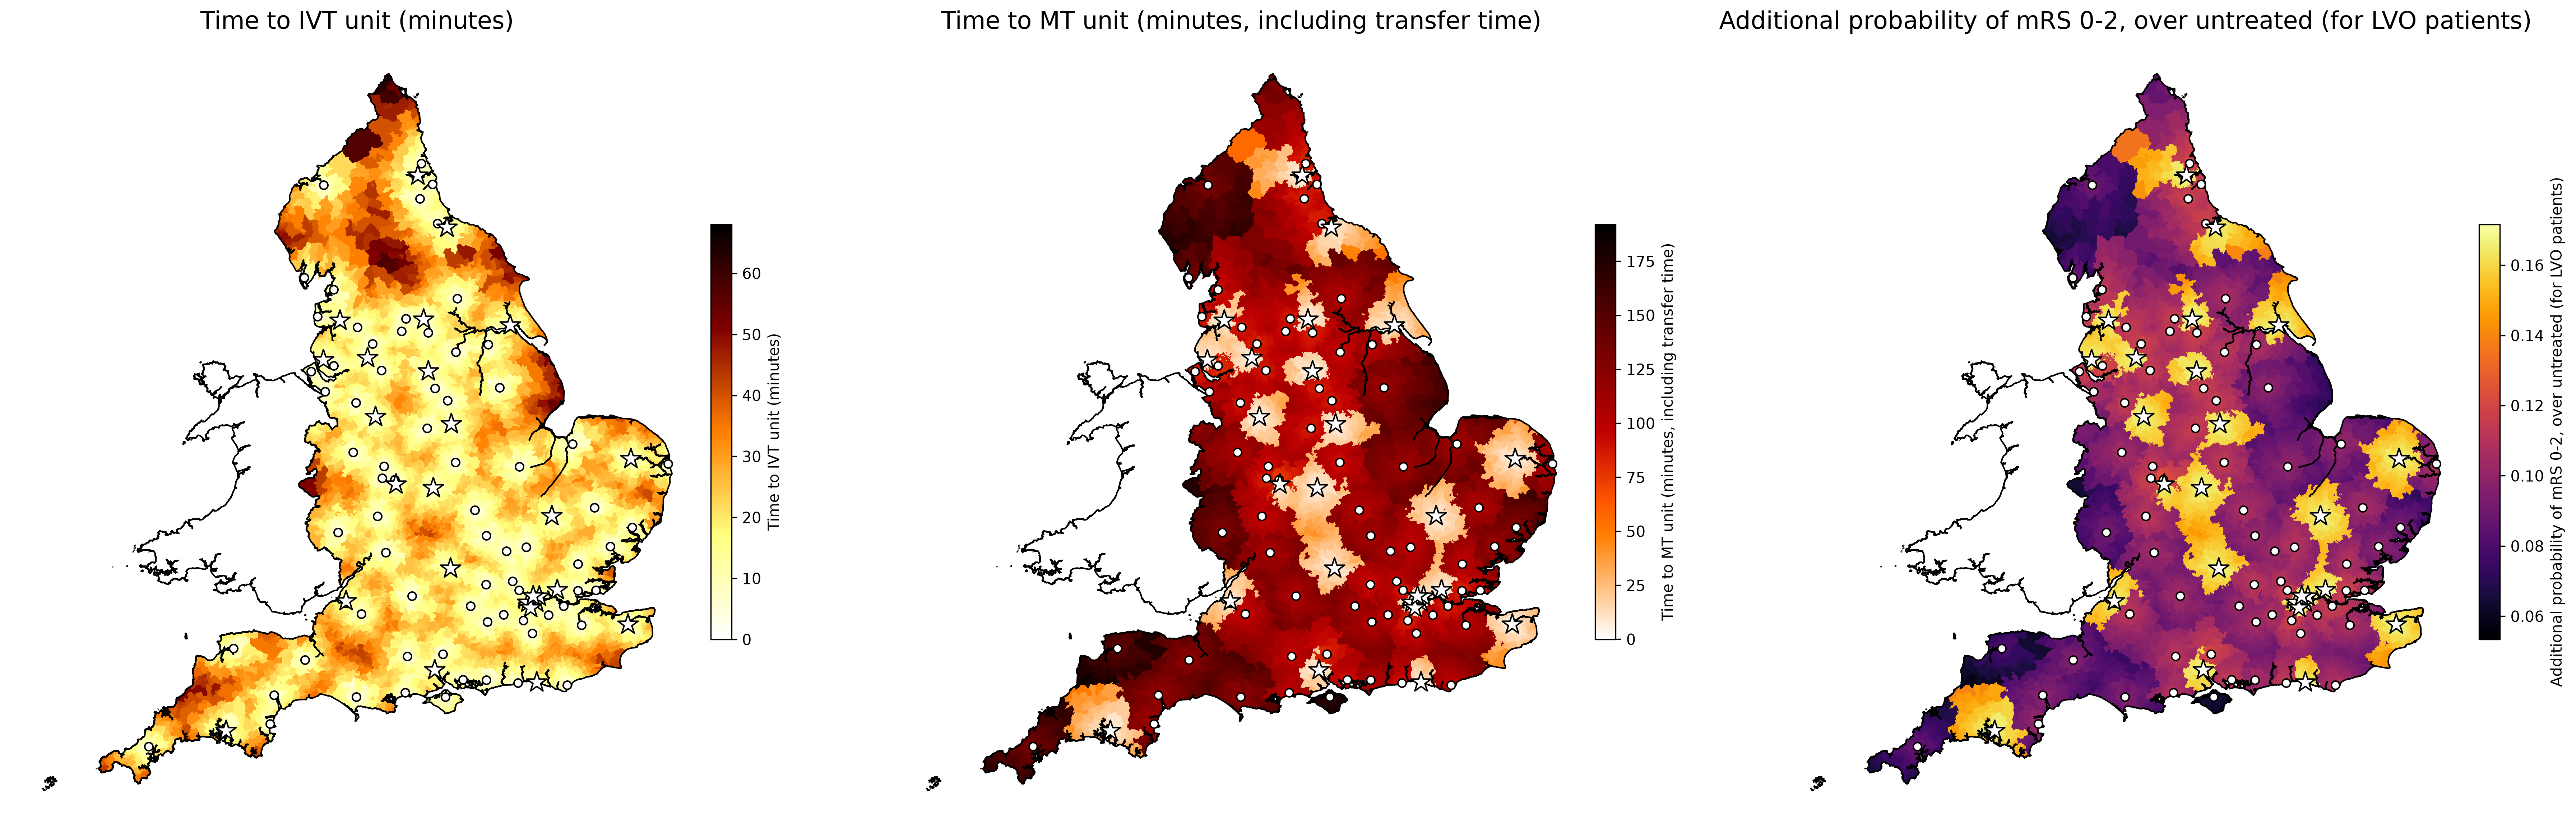
\includegraphics[width=\linewidth]{images/map_three_in_one_current_hospitals_lvo.png} 
\caption{Modelled times and outcomes for stroke patients with large vessel occlusion receiving thrombolysis (IVT) and thrombectomy (MT), with current IVT/MT provision (Taunton and Worcester as IVT-only units) and no loss of MT by first attending an IVT-only unit. \textit{Left}: Predicted travel times to closest (in time) IVT unit. \textit{Middle}: Total travel time to MT unit; this includes travel time to closest IVT unit, a net delay before transfer of 60 minutes, and travel time from IVT unit to MT unit. \textit{Right}: The predicted improvement in the proportion of treated LVO patients with mRS 0-2 at 3-6 months, assuming there is no loss of use of MT by first attending an IVT-only unit. Stroke teams are shown as stars (providing both IVT and MT) or circles (providing IVT alone).}
\label{fig:map_current_no_loss}
\end{figure}

% Base case - loss pf MT
\begin{figure}[H]
\centering
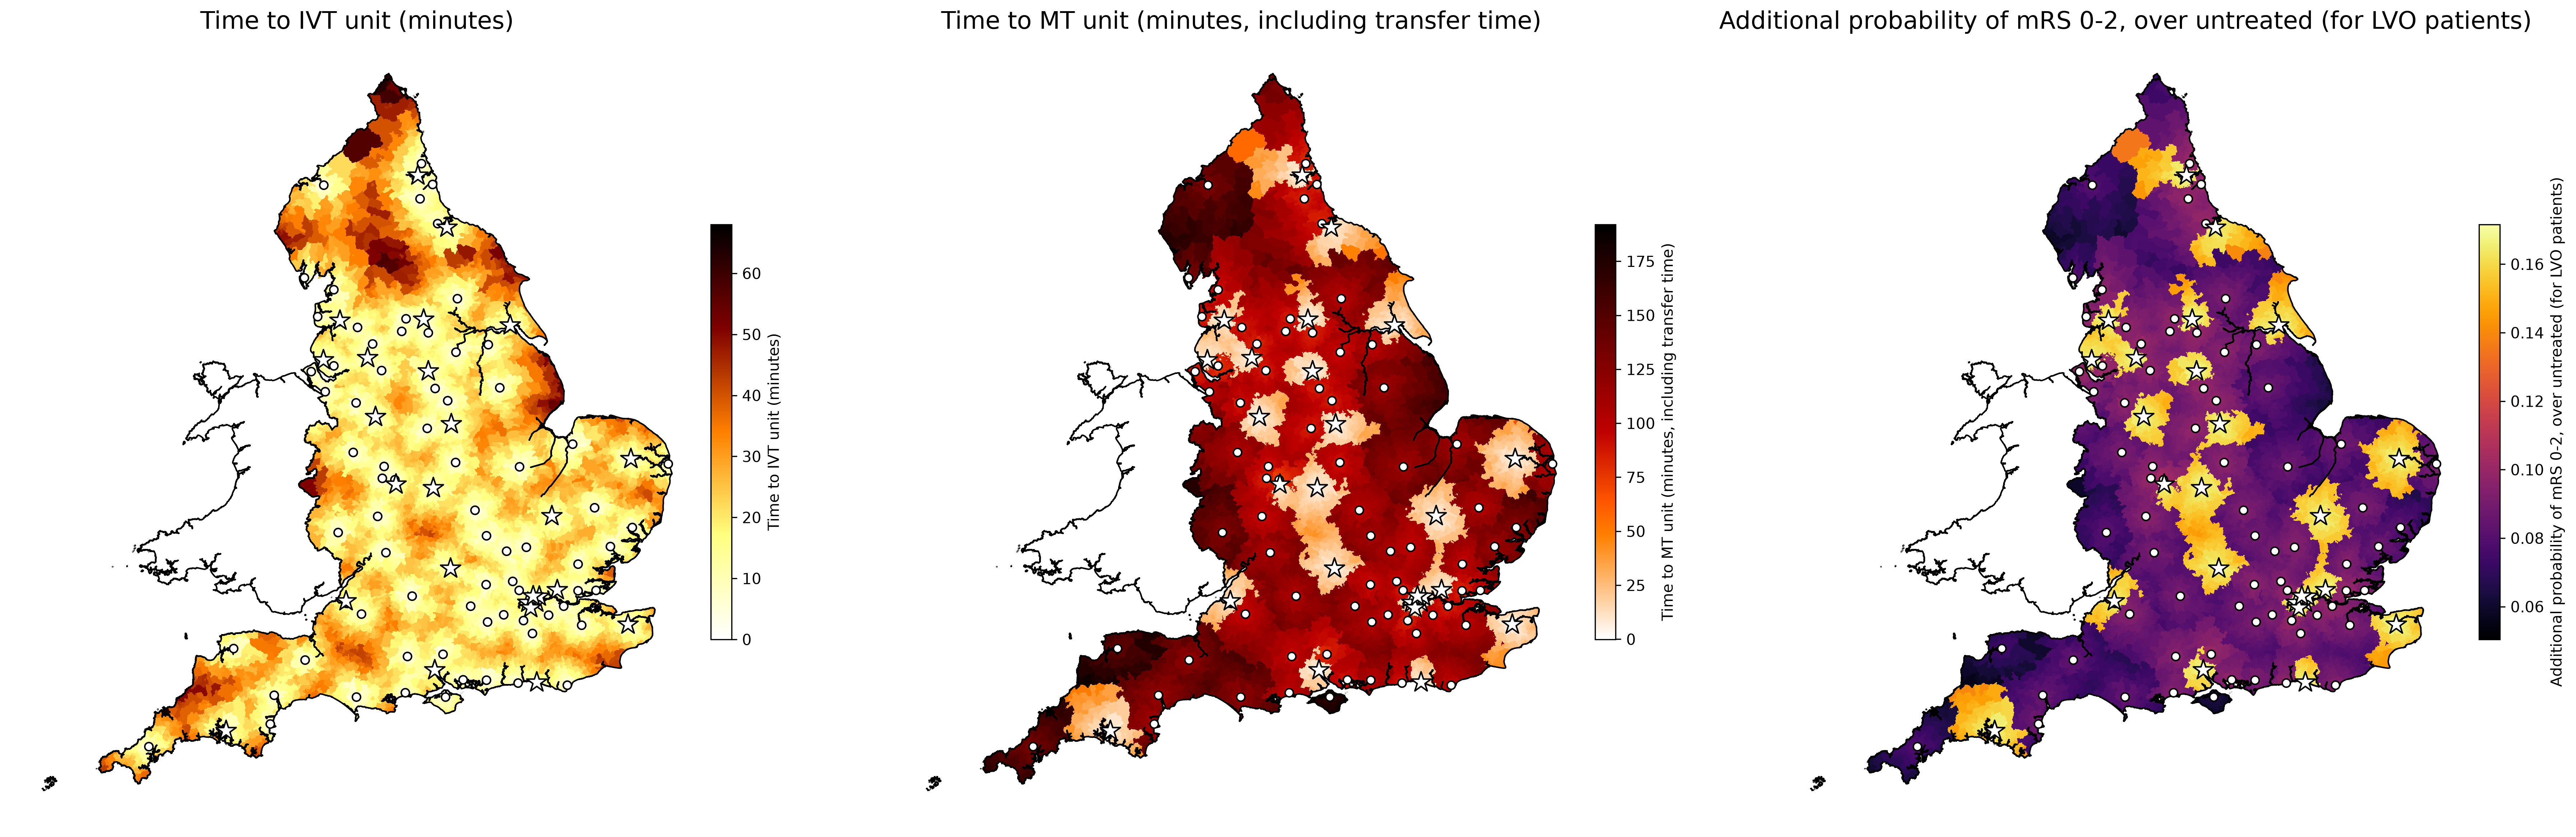
\includegraphics[width=\linewidth]{images/map_three_in_one_current_hospitals_67_percent_transfer_lvo.png} 
\caption{Modelled times and outcomes for stroke patients with large vessel occlusion receiving thrombolysis (IVT) and thrombectomy (MT), with current IVT/MT provision (Taunton and Worcester as IVT-only units) and 33\% loss of use of MT by first attending an IVT-only unit. \textit{Left}: Predicted travel times to closest (in time) IVT unit. \textit{Middle}: Total travel time to MT unit; this includes travel time to closest IVT unit, a net delay before transfer of 60 minutes, and travel time from IVT unit to MT unit. \textit{Right}: The predicted improvement in the proportion of treated LVO patients with mRS 0-2 at 3-6 months, assuming a 33\% loss of use of MT by first attending an IVT-only unit. Stroke teams are shown as stars (providing both IVT and MT) or circles (providing IVT alone).}
\label{fig:map_current_lossy}
\end{figure}


  
% Worcester + Taunton
\begin{figure}[H]
\centering
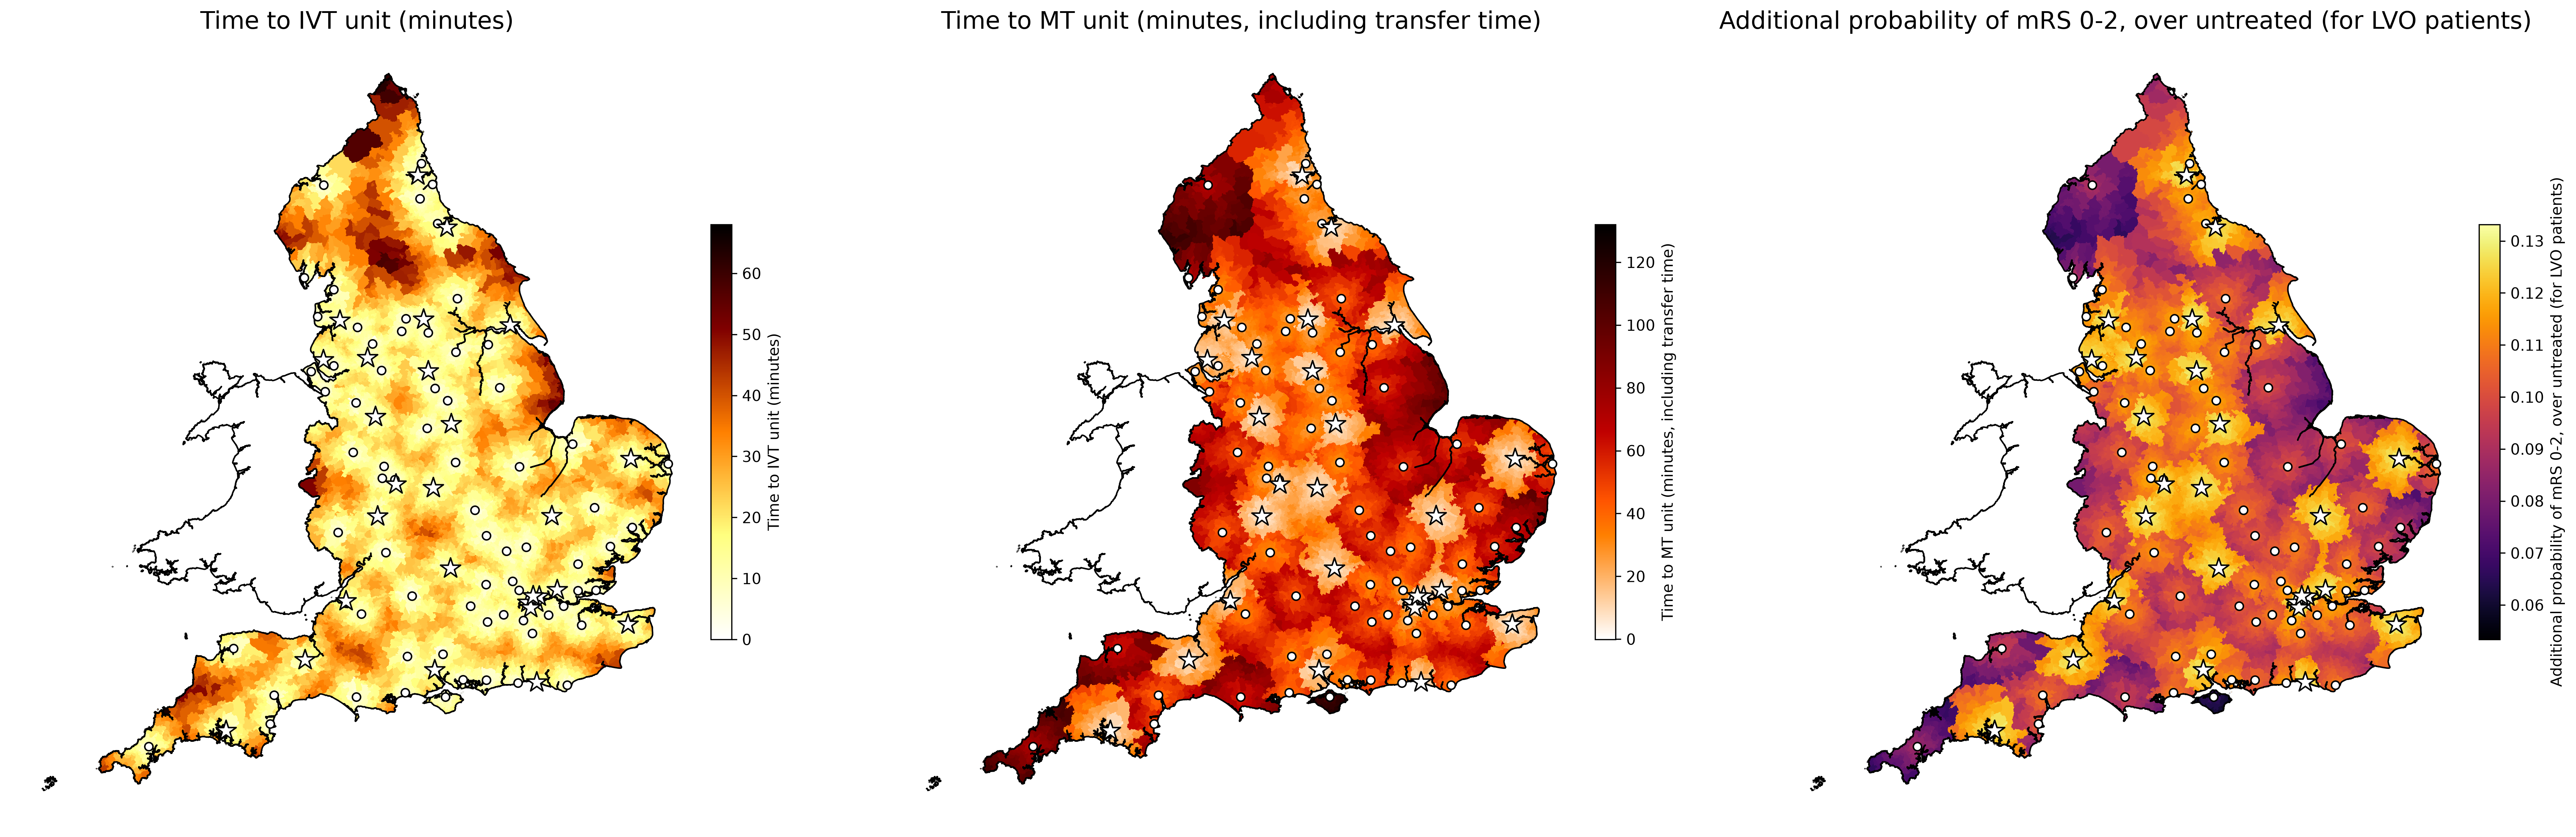
\includegraphics[width=\linewidth]{images/map_three_in_one_taunton_and_worcester_lvo.png}  
\caption{Modelled times and outcomes for stroke patients with large vessel occlusion receiving thrombolysis (IVT) and thrombectomy (MT), with the addition of Taunton and Worcester providing MT, no loss of MT by first attending an IVT-only unit, and with the addition of Taunton and Worcester providing MT. \textit{Left}: Predicted travel times to closest (in time) IVT unit. \textit{Middle}: Total travel time to MT unit; this includes travel time to closest IVT unit, a net delay before transfer of 60 minutes, and travel time from IVT unit to MT unit. \textit{Right}: The predicted improvement in the proportion of treated LVO patients with mRS 0-2 at 3-6 months, assuming there is no loss of use of MT by first attending an IVT-only unit. Stroke teams are shown as stars (providing both IVT and MT) or circles (providing IVT alone).}
\label{fig:map_new_no_loss}
\end{figure}

% Worcester + Taunton - loss pf MT
\begin{figure}[H]
\centering
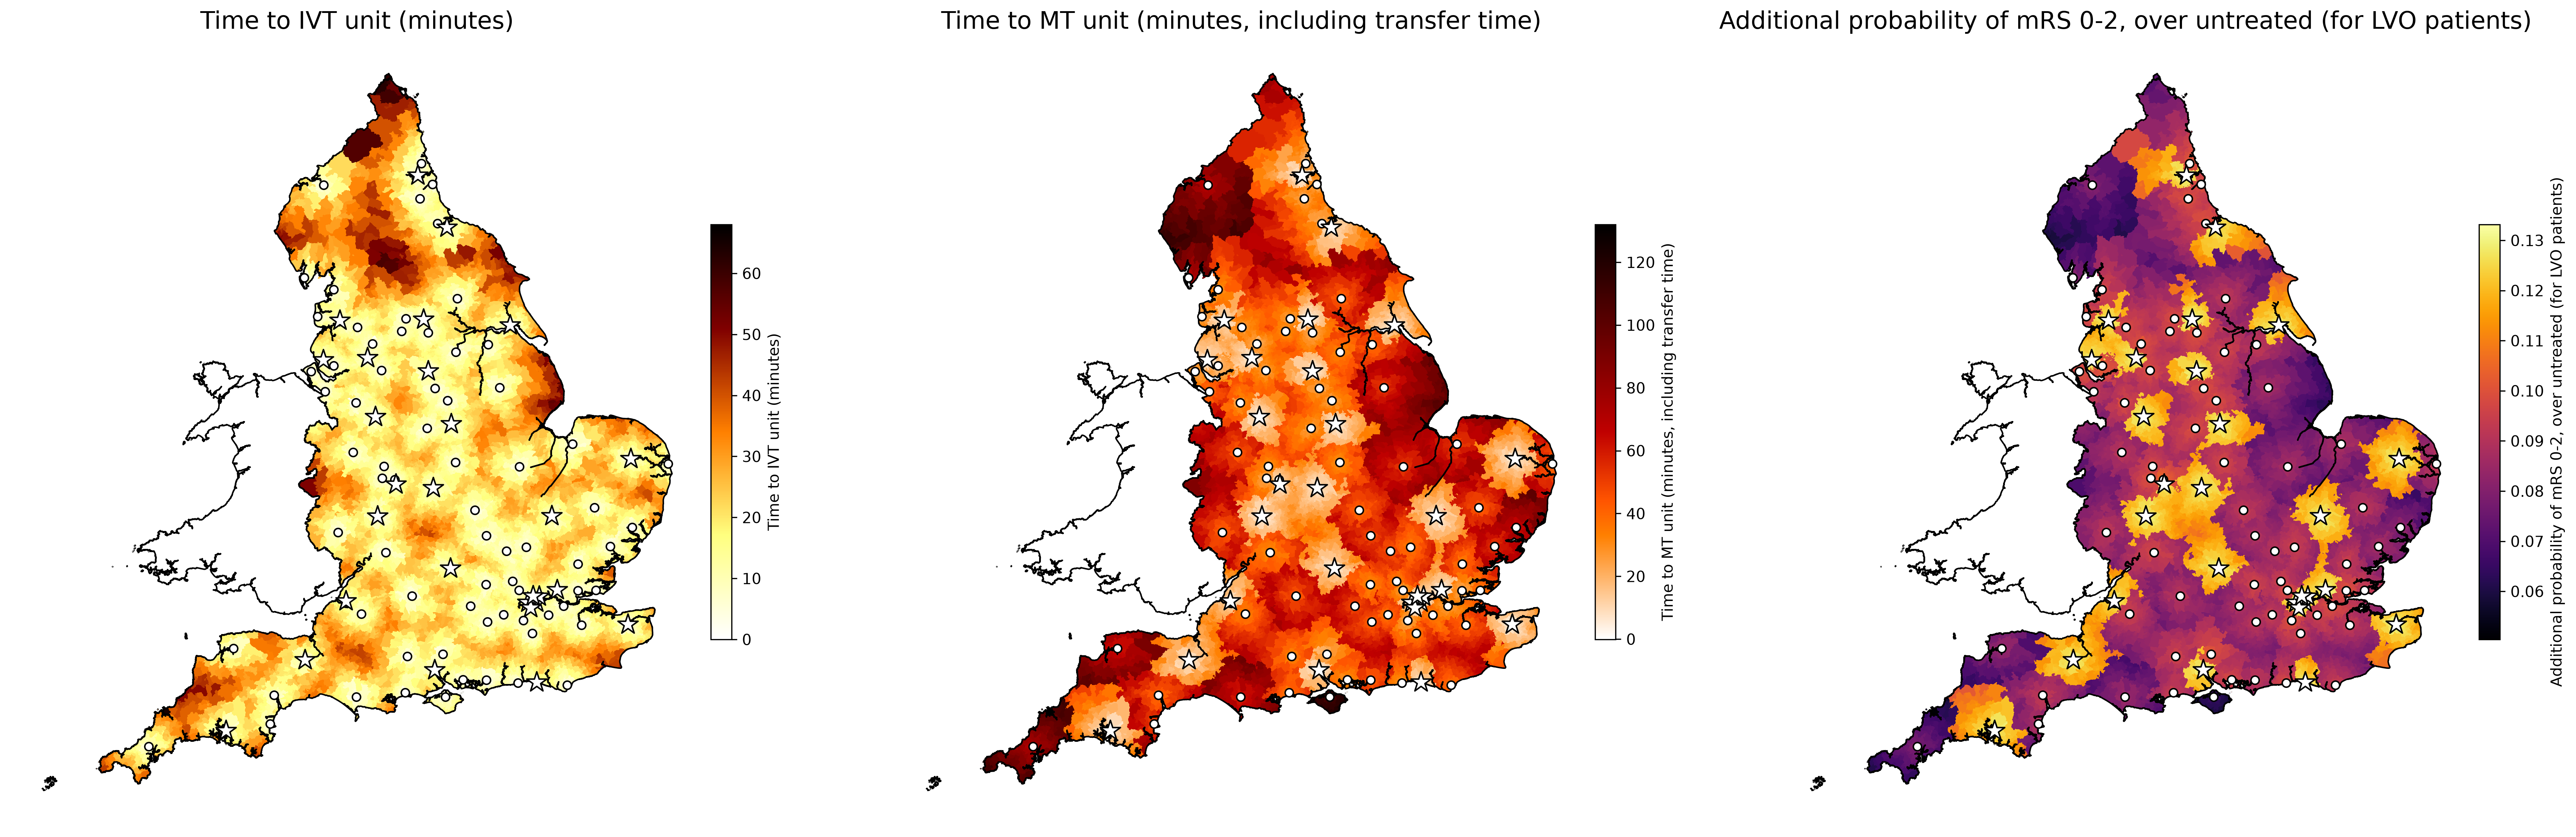
\includegraphics[width=\linewidth]{images/map_three_in_one_taunton_and_worcester_67_percent_transfer_lvo.png} 
\caption{Modelled times and outcomes for stroke patients with large vessel occlusion receiving thrombolysis (IVT) and thrombectomy (MT), with the addition of Taunton and Worcester providing MT, 33\% loss of use of MT by first attending an IVT-only unit, and with the addition of Taunton and Worcester providing MT. . \textit{Left}: Predicted travel times to closest (in time) IVT unit. \textit{Middle}: Total travel time to MT unit; this includes travel time to closest IVT unit, a net delay before transfer of 60 minutes, and travel time from IVT unit to MT unit. \textit{Right}:  The predicted improvement in the proportion of treated LVO patients with mRS 0-2 at 3-6 months, assuming a 33\% loss of use of MT by first attending an IVT-only unit. Stroke teams are shown as stars (providing both IVT and MT) or circles (providing IVT alone).}
\label{fig:map_new_lossy}
\end{figure}


% Comparison maps


\begin{figure}[H]
    \centering
    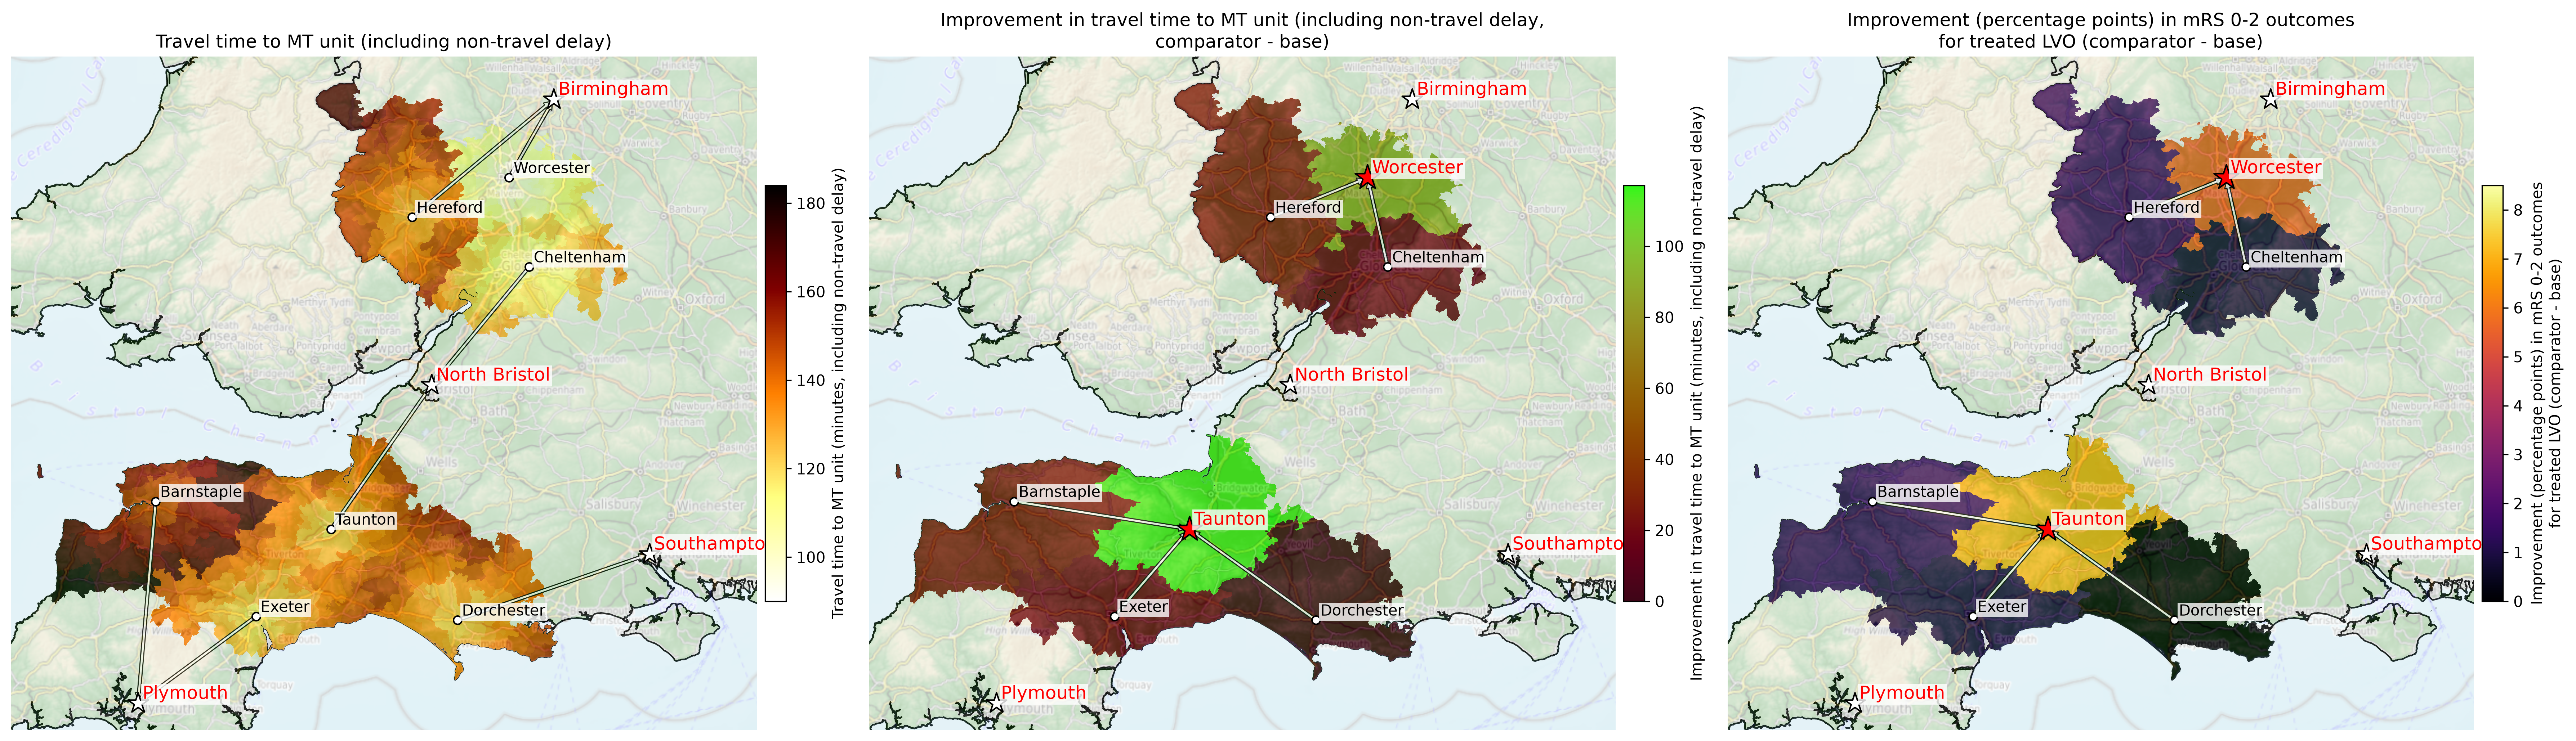
\includegraphics[width=1\linewidth]{images/comparison_map_three_in_one_taunton_worcester.png}
    \caption{Comparison of travel times for MT (including non-travel delays) and outcomes (the predicted improvement in the proportion of treated LVO patients with mRS 0-2 at 3-6 months) by adding MT capability at Taunton and Worcester, with no loss of MT by first attending an IVT-only unit. The arrows indicate the modelled transfer destination from IVT-only units. \textit{Left}: Current predicted travel times for MT, \textit{Middle}: Improvement in travel time to MT. \textit{Right}: Improvement in outcomes.}
    \label{fig:comparison_three_in_one}
\end{figure}

\begin{figure}[H]
    \centering
    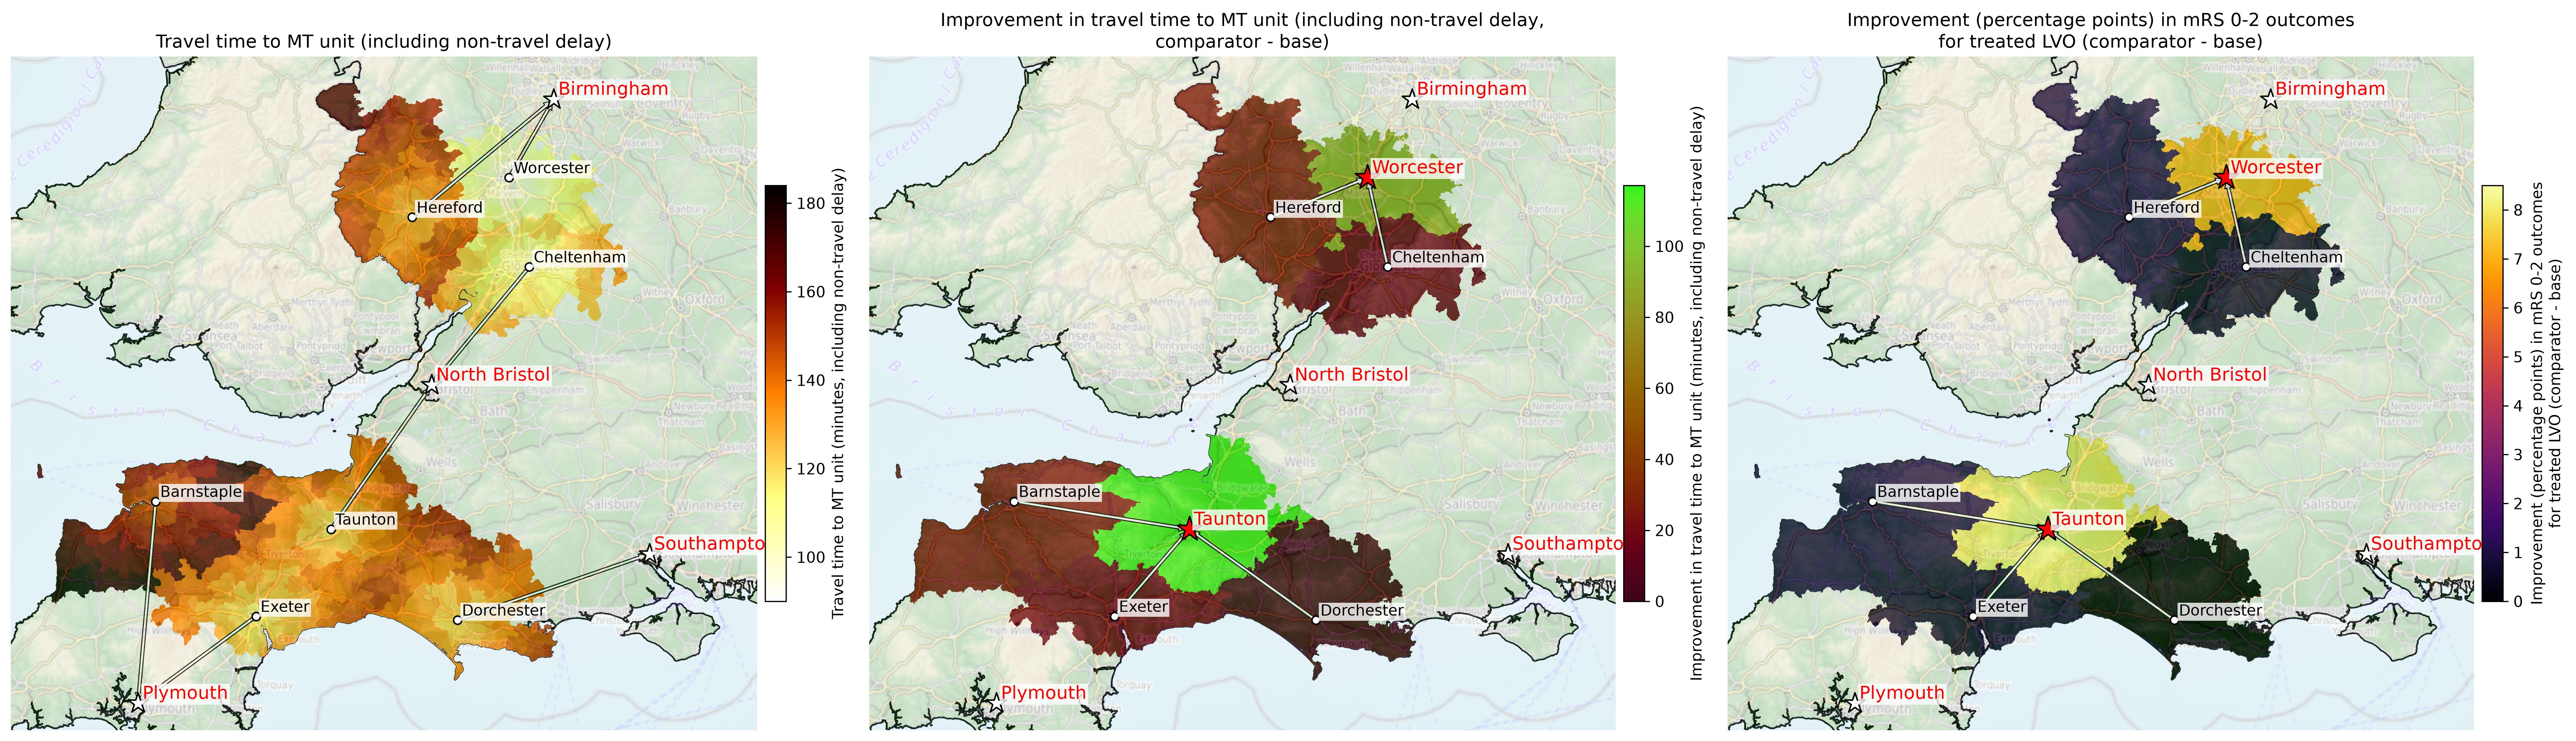
\includegraphics[width=1\linewidth]{images/comparison_map_three_in_one_taunton_worcester_67_percent_transfer.png}
    \caption{Comparison of travel times for MT (including non-travel delays) and outcomes (the predicted improvement in the proportion of treated LVO patients with mRS 0-2 at 3-6 months) by adding MT capability at Taunton and Worcester, with 33\% loss of MT by first attending an IVT-only unit. The arrows indicate the modelled transfer destination from IVT-only units. \textit{Left}: Current predicted travel times for MT, \textit{Middle}: Improvement in travel time to MT. \textit{Right}: Improvement in outcomes.}
    \label{fig:comparison_three_in_one_lossy}
\end{figure}



\subsection{MT admissions of planned system (2 additional MT units)}

Table \ref{tab:mt_units} shows the effect of adding MT units at Taunton and Worcester on MT admissions at MT units in the affected region, if there was no loss of chance to receive MT by first attending an IVT-only unit.

\begin{table}[htbp]
\centering
\caption{Current and planned mechanical thrombectomy (MT) activity by MT unit, including additional MT units at Taunton and Worcester.}
\label{tab:mt_units}
\begin{tabular}{l|c|c|c}
\hline
\textbf{MT Unit} & \textbf{Current MT*} & \textbf{Planned MT*} & \textbf{Change} \\
\hline
Birmingham    & 707 & 585 & $-122$ \\
North Bristol & 393 & 219 & $-174$ \\
Plymouth      & 341 & 231 & $-110$ \\
Southampton**   & 558 & 488 & $-70$  \\
Taunton**     & 0   & 273 & 273    \\
Worcester     & 0   & 202 & 202    \\
\hline
\end{tabular}

\vspace{1.0em}
\begin{minipage}{0.85\linewidth}
\small
*The destination MT unit is chosen as the closest available unit to the first admitting IVT unit. Numbers assume 10\% of all stroke receive MT, with no loss by transfer.\\
**About 70 of Taunton’s MT come from Dorchester (where benefit is negligible compared with current use of Southampton for MT).
\end{minipage}
\end{table}

\subsection{Introducing a travel bias towards selecting an MT unit}

Figures \ref{fig:map_current_bias} and \ref{fig:map_taunton_worcester_bias} show maps of travel times and outcomes for treated LVO patients if patients are taken directly to an MT unit if travel time is no longer than 10 minutes more than first attending a closer IVT-only unit.

For the current provision of MT, a summary of key results is:

\begin{itemize}
    \item Without travel bias, mean percentage point increase in treated LVO with good outcome (mRS 0-2 at 3-6 months) = 12.6 (11.6 with 33\% transfer loss of MT). 33\% admission are direct to MT unit.
    \item With 10 minute travel bias, percentage point increase in treated LVO with good outcome (mRS 0-2 at 3-6 months) = 14.0  (13.4 with 33\% transfer loss of MT). 55\% admission are direct to MT unit.
    \item With 15 minute travel bias, percentage point increase in treated LVO with good outcome (mRS 0-2 at 3-6 months) = 14.8 (14.4 with 33\% transfer loss of MT). 67\% admission are direct to MT unit.
\end{itemize}

With the addition of Taunton and Worcester as MT units, a summary of key results is:

\begin{itemize}
    \item Without travel bias, mean percentage point increase in treated LVO with good outcome (mRS 0-2 at 3-6 months) = 12.7 (11.8 with 33\% transfer loss of MT). 35\% admission are direct to MT unit.
    \item With 10 minute travel bias, percentage point increase in treated LVO with good outcome (mRS 0-2 at 3-6 months) = 14.2  (13.6 with 33\% transfer loss of MT). 57\% admission are direct to MT unit.
    \item With 15 minute travel bias, percentage point increase in treated LVO with good outcome (mRS 0-2 at 3-6 months) = 15.0 (14.6 with 33\% transfer loss of MT). 69\% admission are direct to MT unit.
\end{itemize}

\begin{figure}[H]
    \centering
    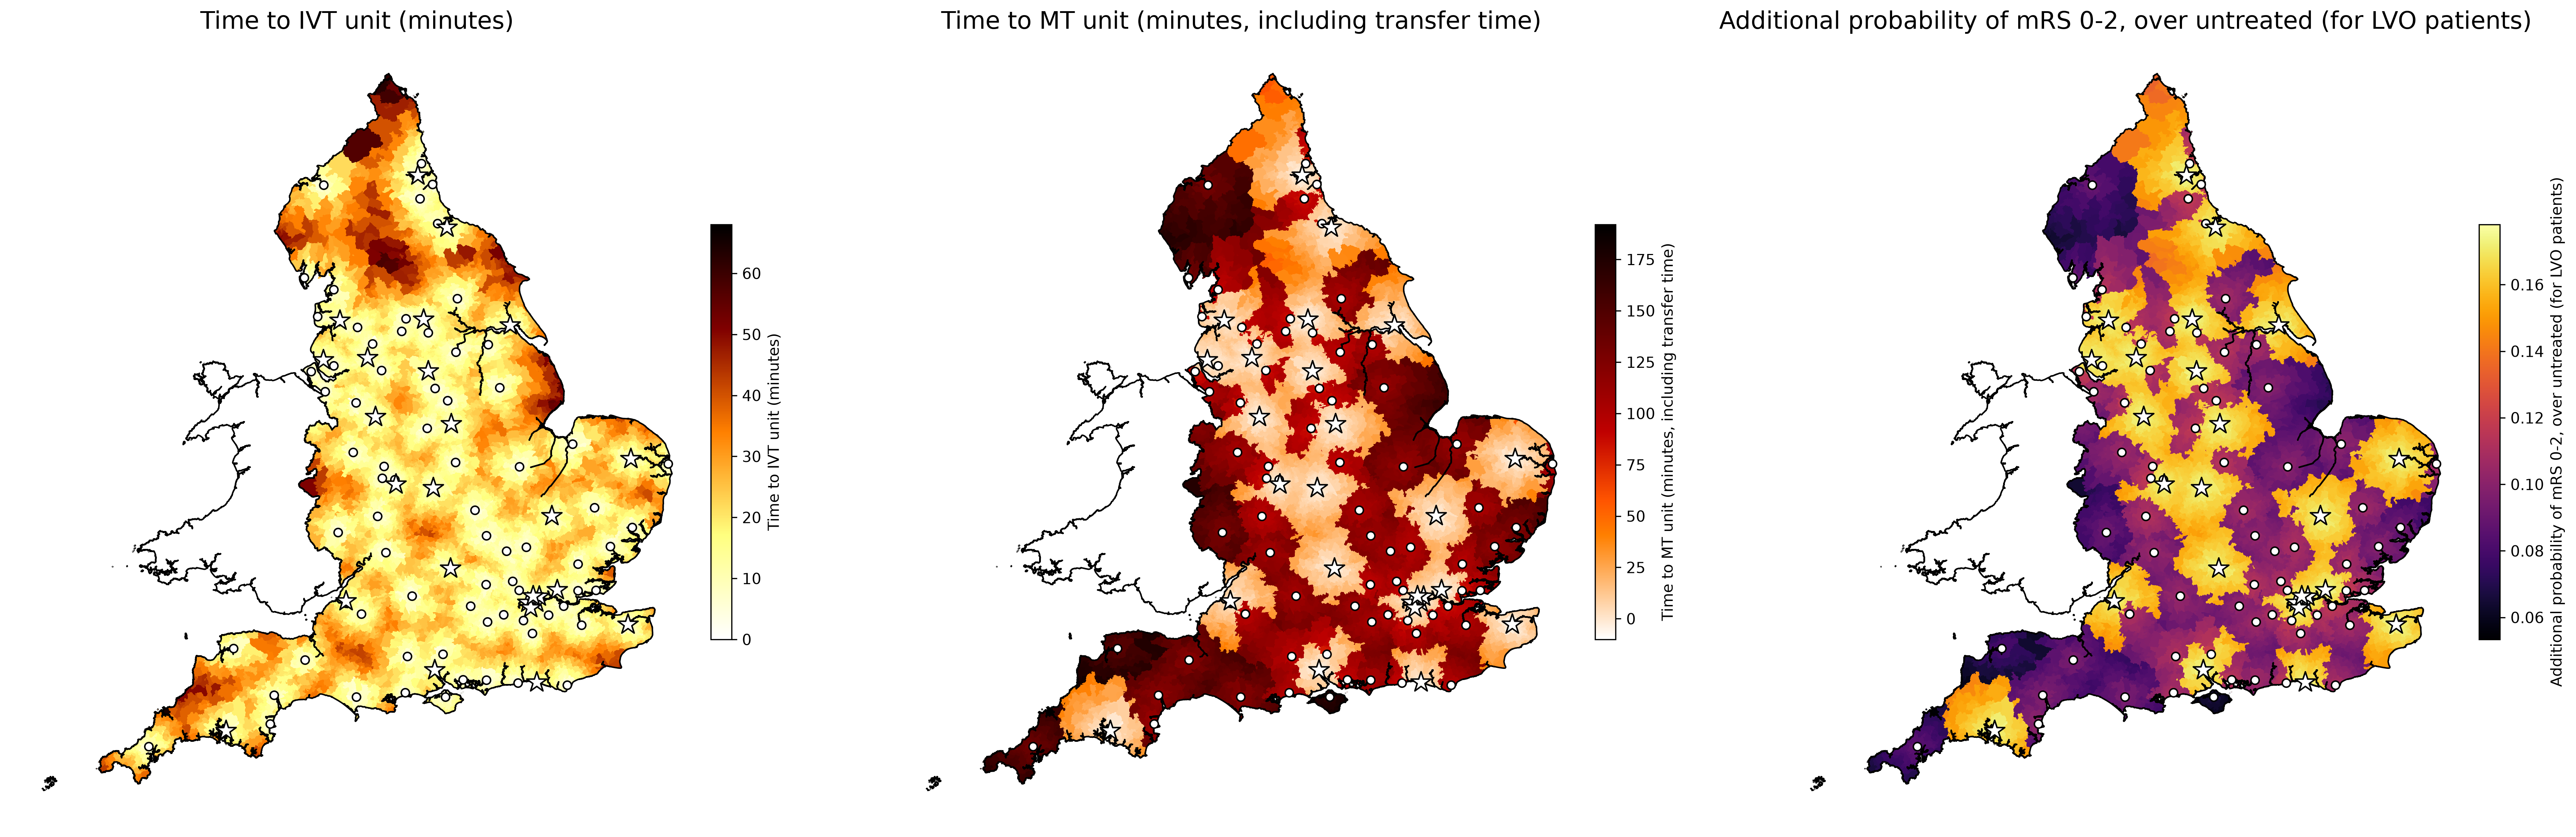
\includegraphics[width=1\linewidth]{images/map_three_in_one_current_hospitals_10min_travel_bias_lvo.png}
    \caption{Modelled times and outcomes for stroke patients with large vessel occlusion receiving thrombolysis (IVT) and thrombectomy (MT), with current IVT/MT provision (Taunton and Worcester as IVT-only units), no loss of MT by first attending an IVT-only unit, and with patients being taken to an MT unit if travel time is no longer than 10 minutes more than first attending a closer IVT-only unit. \textit{Left}: Predicted travel times to closest (in time) IVT unit. \textit{Middle}: Total travel time to MT unit; this includes travel time to closest IVT unit, a net delay before transfer of 60 minutes, and travel time from IVT unit to MT unit. \textit{Right}: The predicted improvement in the proportion of treated LVO patients with mRS 0-2 at 3-6 months, assuming there is no loss of use of MT by first attending an IVT-only unit. Stroke teams are shown as stars (providing both IVT and MT) or circles (providing IVT alone).}
    \label{fig:map_current_bias}
\end{figure}

\begin{figure}[H]
    \centering
    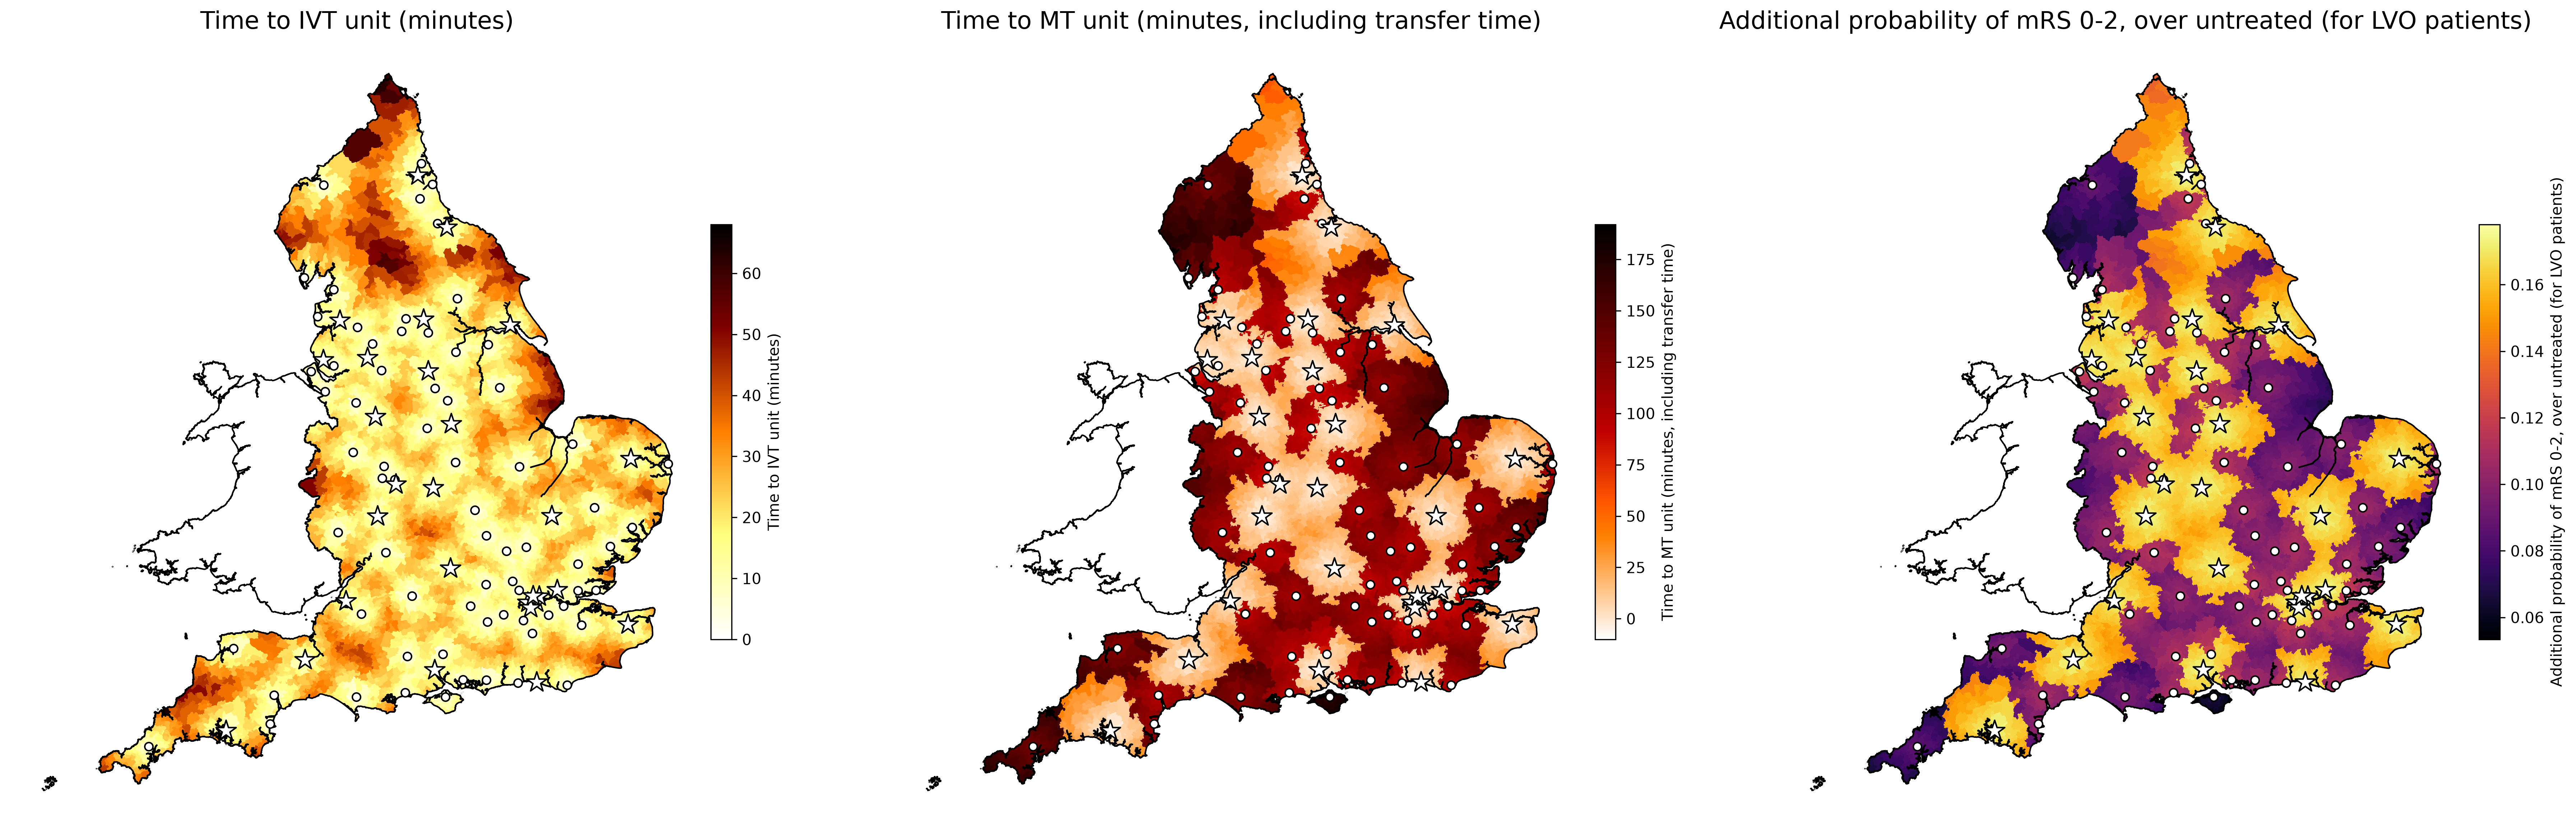
\includegraphics[width=1\linewidth]{images/map_three_in_one_taunton_and_worcester_10min_bias_lvo.png}
    \caption{Modelled times and outcomes for stroke patients with large vessel occlusion receiving thrombolysis (IVT) and thrombectomy (MT), with the addition of Taunton and Worcester providing MT, no loss of MT by first attending an IVT-only unit, and with patients being taken to an MT unit if travel time is no longer than 10 minutes more than first attending a closer IVT-only unit. \textit{Left}: Predicted travel times to closest (in time) IVT unit. \textit{Middle}: Total travel time to MT unit; this includes travel time to closest IVT unit, a net delay before transfer of 60 minutes, and travel time from IVT unit to MT unit. \textit{Right}: The predicted improvement in the proportion of treated LVO patients with mRS 0-2 at 3-6 months, assuming there is no loss of use of MT by first attending an IVT-only unit. Stroke teams are shown as stars (providing both IVT and MT) or circles (providing IVT alone).}
    \label{fig:map_taunton_worcester_bias}
\end{figure}